%version of 07-03-19

\chapter{PAIRING FUNCTIONS: Encoding $\N^+ \times \N^+$ as $\N^+$}
\label{Appendix:building-pairing-functions}

This chapter extends our coverage of pairing functions in
Section~\ref{sec:pairing} by describing a variety of specific such
functions, in the spirit of Section~\ref{sec:diag-pair-fn}.  Our
motivation is twofold.  On the one hand, the mathematics needed to
verify the bijectiveness of the functions we discuss provides valuable
practice with some of the tools we have been developing until now.  On
the other hand, the manifold varied applications of pairing functions
adds value to our excursion into the world of these functions.  The
detailed survey article \cite{Rosenberg03} provides much more detail
than we are able to provide here.

\bigskip

As we embark on our very short guided tour, the reader should note
that the diagonal pairing function of Section~\ref{sec:diag-pair-fn}
and the square-shell pairing function of
Section~\ref{sec:square-pair-fn} build in essential ways on the
$L$-norms of Section~\ref{sec:Ln-norms}; cf., Fig.~\ref{fig:Ln-discs}.

\ignore{*************
{\Denis The introduction has been taken from the main part of the book,
it has to be rewritten}

The remainder of this section is devoted to developing {\em easily
  computed} bijections between the set $\N^+ \times \N^+$ and the set
$\N^+$ of positive integers.  We thereby exhibit easily computed
mechanisms for \underline{encoding} ordered pairs of integers---hence,
also, tuples, strings, and binary trees of integers---as single
integers.  We thereby see that---at least within the world of integers
and entities encodable as integers---there is no intrinsic new power
inherent in tuple-spaces: \index{tuple-spaces} {\em Sets of tuples of
  integers can be efficiently encoded as sets of integers.}  Because
of the special role of ordered pairs of integers in our study of
encodings of structured sets of integers---they form the fundamental
puzzle from whose solution all else will follow---a special name has
been associated with bijections between $\N^+ \times \N^+$ and $\N^+$.
These special bijections are called {\it pairing functions}.
\index{pairing functions!encodings}

One of the most valuable by-products of encodings provided by pairing
functions is that such encodings provide {\em linear orderings} of the
\index{pairing functions!linear orderings}
set being encoded.  We noted in Section~\ref{sec:integers}.A that
``order within a number system is among one's biggest friends when
reasoning about the numbers within the system.''  The orderings
provided by these encodings are particularly
valuable when the structured sets being encoded as integers do not
have their own ``intrinsic'' or ``natural'' orderings.  Included in
this category are  structures such as tuples,
strings, and trees.
\bigskip

\noindent \fbox{
\begin{minipage}{0.95\textwidth}
Of course some structured sets do have natural, native linear orders:
consider, as one such, strings under lexicographic ordering.  Even for
such sets, we often benefit from having alternative orderings as we
design and analyze algorithms on the sets.
\end{minipage}
}
\bigskip
***************}

\section{A Shell-Based Methodology for Crafting Pairing Functions}
\label{sec:build-pair-fn}
\index{constructing pairing functions via ``shells''}
\index{pairing functions as storage mappings for arrays/tables}

The shell-oriented strategy that underlies the diagonal pairing
function $\d$ can be adapted to incorporate shell-``shapes'' that are
inspired by a variety of computational situations---and can be applied
to great computational advantage in such situations.  We describe how
such adaptation can be effected, and we describe a few explicit shapes
and situations.  We invite the reader to craft others.

\medskip

{\Denis Change the style for writing the algorithms -- We should guarantee the coherency all over the book!}

\noindent {\underline{\bf Procedure}} {\small\sf PF-Constructor}($\a$) \\
/*Construct a shape-inspired pairing function (PF) $\a$*/
\begin{description}
\item[Step 1.]
%
Partition the set $\N^+ \times \N^+$ into finite sets called {\it
  shells}.  Order the shells linearly in some way: many natural
shell-partitions carry a natural order.
\end{description}
As noted above, Shell $c$ of the diagonal pairing function $\d$ is the
following subset of $\N^+ \times \N^+$: $\{ \langle x,y \rangle \ |
\ x+y = c \}$.  The parameter $c$ orders $\d$'s shells.

\begin{description}
\item[Step 2.]
Construct a pairing function from the shells as follows.
  \begin{description}
  \item[Step 2a.]
Enumerate $\N^+ \times \N^+$ shell by shell, honoring the ordering of
the shells; i.e., list the pairs in shell \#1, then shell \#2, then
shell \#3, etc.
  \item[Step 2b.]
Enumerate each shell in some systematic way, e.g., ``by columns'':
Enumerate the pairs $\langle x,y \rangle$ in each shell in increasing
order of $y$ and, for pairs having equal $y$ values, in decreasing
order of $x$.
  \end{description}
\end{description}

\begin{prop}
\label{thm:PF-construct}
Any function $\a: \N^+ \times \N^+ \leftrightarrow \N^+$ that is
designed via Procedure {\small\sf PF-Constructor} is a bijection.
\end{prop}

\begin{proof}(Sketch) Step 1 of Procedure {\small\sf PF-Constructor}
constructs a partial order on $\N^+ \times \N^+$, in which: ($a$) each
shell is finite; ($b$) there is a linear order on the shells.  Step 2
extends this partial order to a linear order, by honoring the inherent
ordering of shells and imposing a linear order within each shell.  The
function constructed via the Procedure is: {\em injective} because the
disjoint shells are enumerated sequentially; {\em surjective} because
the enumeration within each shell begins immediately after the
enumeration within the preceding shell, with no gap.  \qed
\end{proof}

\bigskip

We have noted how to use Procedure {\small\sf PF-Constructor} to
construct pairing function $\d$.  We now use the Procedure to design
two other useful pairing functions.

\section{The Square-shell Pairing Function $\s$}
\label{sec:square-pair-fn}
\index{The Square-shell pairing function $\s$}

One computational situation where pairing functions can be useful
involves storage-mappings for arrays/tables that can expand and/or
contract dynamically.  In conventional systems, when one expands an $n
\times n$ table into an $(n+1) \times (n+1)$ table, one allocates a
new region of $(n+1)^2$ storage locations and copies the current table
from its $n^2$-location region to the new region.  Of course, this is
very wasteful: one is moving $\Omega(n^2)$ items to make room for the
anticipated $2n+1$ new items.  On any given day, the practical impact
of this waste depends on current technology.  But, this is a
mathematics text, not an engineering one, so we are exploring whether
{\em in principle} we can avoid the waste.  The answer is ``YES''.  If
we employ a pairing function $\varepsilon: \N^+ \times \N^+
\leftrightarrow \N^+$ to allocate storage for tables, then to expand a
table from dimensions $n \times n$ to $(n+1) \times (n+1)$, we need
move only $O(n)$ items to accommodate the {\em new} table entries; the
current entries need not be moved.  For square tables, the following
{\it Square-shell} pairing function $\s$ manages the described
scenario perfectly.  After describing $\s$, we comment on managing
tables of other shapes.
\begin{figure}[htb]
\begin{center}
%\begin{tabular}{r|r|r|r|r|r|r|r|r}
%  1 &  4 &  9 & 16 & \fbox{25} &  36 &  49 &  64 & $\cdots$ \\
%  2 &  3 &  8 & 15 & \fbox{24} &  35 &  48 &  63 & $\cdots$ \\
%  5 &  6 &  7 & 14 & \fbox{23} &  34 &  47 &  62 & $\cdots$ \\
% 10 & 11 & 12 & 13 & \fbox{22} &  33 &  46 &  61 & $\cdots$ \\
%\fbox{17} & \fbox{18} & \fbox{19} & \fbox{20} & \fbox{21} &  32 &  45
%  &  60 & $\cdots$ \\ 
% 26 & 27 & 28 & 29 & 30 &  31 &  44 &  59 & $\cdots$ \\
% 37 & 38 & 39 & 40 & 41 &  42 &  43 &  58 & $\cdots$ \\
% 50 & 51 & 52 & 53 & 54 &  55 &  56 &  57 & $\cdots$ \\
%$\vdots$ & $\vdots$ & $\vdots$ & $\vdots$ & $\vdots$ & $\vdots$ &
%  $\vdots$ & $\vdots$ & $\ddots$
%\end{tabular}
   \includegraphics[scale=0.4]{FiguresArithmetic/PairingSquareShell}
\end{center}
\caption{{\it The square-shell pairing function $\s$.  The shell
    $\max(x,y) = 5$ is highlighted.}
\label{fig:pairingSquareShell}}
\end{figure}
\begin{equation}
\label{e.square}
\begin{array}{ccl}
\s(x, y) & = & m^2 + m + y-x+1 \\
 & & \mbox{where } \ \ \  m \ \eqdef \ \max(x-1,y-1).
\end{array}
\end{equation}
One sees in Fig.~\ref{fig:pairingSquareShell} that $\s$ follows the
prescription of Procedure PF-Constructor: (1) it maps integers into
the ``square shells'' defined by: $m = 0, \ m = 1, ...$.  (2) it
enumerates the entries in each shell in a counterclockwise direction.
(Of course, $\s$ has a twin that enumerates the shells in a clockwise
direction.)
\bigskip

\noindent \fbox{
\begin{minipage}{0.95\textwidth}
Using somewhat more complicated instantiations of Procedure
  PF-Constructor, the study in \cite{Rosenberg75} adapts the
  square-shell pairing function $\s$ to: ($a$) accommodate, with no
  wastage, arrays/tables of any fixed aspect ratio $an \times bn$
  ($a,b \in \N$); ($b$) accommodate, with only $O(n)$ wastage,
  arrays/tables whose aspect ratios come from a fixed finite set of
  candidates---i.e., $(a_1 n \times b_1 n)$ or $(a_2 n \times b_2 n)$
  or \ldots or $(a_k n \times b_k n)$.
\end{minipage}
}

\section{$\oplus$ The Hyperbolic-Shell Pairing Function $\h$}
\label{Appendix:hyp-shell-pair-fn}
\index{The Hyperbolic-shell pairing function $\h$}

We have just seen, in subsections B and C, that when the growth
patterns of one's arrays/tables is very constrained, one can use
pairing functions as storage mappings with very little wastage.  In
contrast, if one employs a pairing function such as $\d$ without
consideration of its wastage, then a storage map would show some
$O(n)$-entry tables being ``spread'' over $\Omega(n^2)$ storage
locations.  In the worst-case, $\d$ spreads the $n$-position $1 \times
n$ array/table over $> {1 \over 2} n^2$ addresses: $\d(1,1) = 1$ and
$\d(1,n) = {1 \over 2} (n^2 + n)$.  This degree of wastefulness can be
avoided via careful analysis, coupled with the use of Procedure
PF-Constructor.  The target commodity to be minimized is the {\it
  spread} of a PF-based storage map, which we define as follows.
\index{the spread of a pairing function}

Note that an ordered pair of integers $\langle x,y \rangle$ appears as
a position-index within an $n$-position table if, and only if, $xy
\leq n$.  Therefore, we define the spread of a PF-based storage map
$\m$ via the function
\begin{equation}
\label{e.compact}
{\bf S}_{\cal M}(n) \ \eqdef \ \max\{ \m(x, y) \ | \ xy \leq n \}.
\end{equation}
${\bf S}_{\cal M}(n)$ is the largest ``address'' that PF $\m$ assigns
to any position of a table that has $n$ or fewer positions.

Happily, the tools we have developed enable us to design a pairing
function that (to within constant factors) has minimum worst-case
spread.  This is the {\em Hyperbolic-shell pairing function} $\h$ of
(\ref{e.hyper}) and Fig.~\ref{fig:pairingHyper}.\footnote{Details appear in
  \cite{Rosenberg74,Rosenberg75}.}
\begin{equation}
\label{e.hyper}
\begin{array}{lcll}
\multicolumn{4}{l}{\mbox{Let $\delta(k)$ be the number of divisors of
    the integer $k$.}} \\
\h(x,y) & = & {\displaystyle \sum_{k=1}^{xy-1} \delta(k) \ \ +} &
  \mbox{the position of } \ \langle x, y \rangle \ \mbox{ among 2-part} \\
        &   &  & \mbox{factorizations of the number $xy$, in} \\
        &   &  & \mbox{reverse lexicographic order}
\end{array}
\end{equation}
\begin{figure}[htb]
\begin{center}
%\begin{tabular}{r|r|r|r|r|r|r|r}
% 1 &  3 &  5 &   8 &  10 & \fbox{14} &  16  & $\cdots$ \\
% 2 &  7 & \fbox{13} &  19 &  26 &  34 &  40 & $\cdots$ \\
% 4 & \fbox{12} & 22 &  33 &  44 &  56 &  69 & $\cdots$ \\
% 6 & 18 & 32 &  48 &  64 &  81 &  99  & $\cdots$ \\
% 9 & 25 & 43 &  63 &  86 & 108 & 130  & $\cdots$ \\
%\fbox{11} & 31 & 55 &  80 & 107 & 136 & 165 & $\cdots$ \\
%15 & 39 & 68 &  98 & 129 & 164 & 200  & $\cdots$ \\
%17 & 47 & 79 & 116 & 154 & 193 & 235  & $\cdots$ \\
%$\vdots$ & $\vdots$ & $\vdots$  & $\vdots$ & $\vdots$ &
%  $\vdots$ & $\vdots$ & $\ddots$
%\end{tabular}
      \includegraphics[scale=0.4]{FiguresArithmetic/PairingHyper}
\end{center}
\caption{{\it The hyperbolic pairing function $\h$.  The shell $xy = 6$ is
highlighted.}
\label{fig:pairingHyper}}
\end{figure}


\begin{prop}[\cite{Rosenberg75}]
\label{thm:hyp-opt}
{\bf (a)}
The hyperbolic function $\h$ is a pairing function.

\noindent {\bf (b)}
The spread of $\h$ is given by
${\bf S}_{\cal H}(n) \ = \ O(n \log n)$.\footnote{A  detailed
  analysis reveals that the spread of $\cal H$ is closely related to
  the {\em natural} logarithm, whose base is Euler's constant $e$.}

\noindent {\bf (c)}
No pairing function has better compactness than $\h$ (in the worst
case) by more than a constant factor.
\end{prop}

\begin{proof}
{\bf (a)} The fact that $\h$ is a pairing function follows from
Proposition~\ref{thm:PF-construct}.

\noindent {\bf (b)}
The pairing function $\h$ maps integers along the ``hyperbolic
shells'' defined by $xy = 1, \ xy =2, \ xy=3, \ldots$.  Hence,
when an integer $n$ is ``placed'' into the table of values of
$\h$, the number of occupied slots is within $n$ of
\[ \sum_{i=1}^{n-1} \ |\{ \langle x,y \rangle \ | \ xy < i \}| 
\]
Elementary calculations show that this sum is $O(n \log n)$.

\noindent {\bf (c)} The optimality of $\h$ in compactness (up to
constant factors) is seen via the following argument.  The set of
tables that have $n$ or fewer positions are those of aspect ratios
$a_i \times b_i$, where $a_i b_i \leq n$.  As one sees from
Fig.~\ref{f.hyp} (generalized to arbitrary $n$), the union of the
positions of all these arrays is the set of integer lattice points
under the hyperbola $xy = n$.  It is
well-known---cf.~\cite{NivenZ80}---that this set of points has
cardinality $\Theta(n \log n)$.\footnote{Recall from
  Chapter~\ref{sec:set-concepts} that the {\it cardinality} of a
  finite set $S$ is the number of elements in $S$.}  Since every table
contains position $\langle 1,1 \rangle$, it follows that, for every
$n$, some table containing $n$ or fewer positions is spread over
$\Omega(n \log n)$ ``addresses.''  \qed
\end{proof}
\begin{figure}[htb]
\begin{center}
       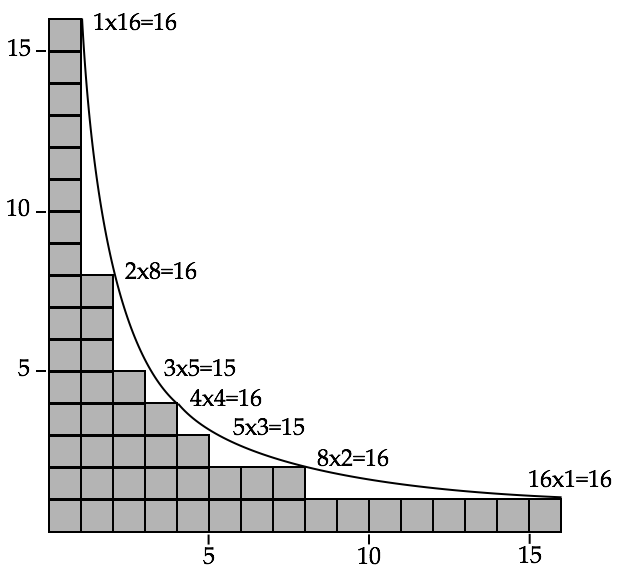
\includegraphics[scale=0.4]{FiguresArithmetic/PairingHyp}
\caption{The aggregate set of positions of tables having $16$ or
    fewer position.  To help the reader understand the figure, we
    include the curve $f(x,y) = xy$ which provides an upper envelope
    for the set.  A careful look at this curve will reveal that it
    touches the set of positions at the points $\langle x,y \rangle
    \in \{ \langle 1,16 \rangle, \ \langle 2,8 \rangle, \ \langle 4,4
    \rangle, \ \langle 8,2 \rangle, \ \langle 16,1 \rangle \}$, but it
    does {\em not} touch the set at the points $\langle x,y \rangle
    \in \{ \langle 3,5 \rangle, \ \langle 5,3 \rangle \}$. 
\label{f.hyp}}
\end{center}
\end{figure}

\section{A Pairing Function Built from Disjoint Arithmetic Progressions}

As we noted earlier, the notion of pairing function has applications
to a broad range of computational situations.  For some of
these---cf., \cite{Rosenberg03}---it is convenient to have each
``row'' of the pairing function map onto an arithmetic progression.
This can be achieved in many ways, as explained in \cite{Rosenberg03}.
For this chapter, we satisfy ourselves with presenting a single such
{\em additive} pairing function, let us call it $\a(x,y)$.

For all $\langle x,y \rangle \in \N^+ \times \N^+$

$\a(x,y) \ \eqdef \ 2^{x-1} \cdot (2y -1)$

We leave to the reader the exercise of verifying function $\a$'s
bijectiveness.  As an aid, we provide the following prefix of $\a$'s
mapping of $\N^+ \times \N^+$.
\begin{center}
\begin{tabular}{r|r|r|r|r|r|r}                                                               
 1 &  3 &   5 &   7 &   9 &  11 & $\cdots$ \\                                      
 2 &  6 &  10 &  14 &  18 &  22 & $\cdots$ \\                                      
 4 & 12 &  20 &  28 &  36 &  44 & $\cdots$ \\                                      
 8 & 24 &  40 &  56 &  72 &  88 & $\cdots$ \\                                            
16 & 48 &  80 & 112 & 144 & 176 & $\cdots$ \\
32 & 96 & 110 & 224 & 288 & 352 & $\cdots$ \\                                      
$\vdots$ & $\vdots$ & $\vdots$  & $\vdots$ & $\vdots$ & $\vdots$ & $\ddots$
\end{tabular} 
\end{center}
